%chktex-file 36
%chktex-file 23
%chktex-file 10
%chktex-file 17
%chktex-file 9
\documentclass[computationalMathematics.tex]{subfiles}

\begin{document}

%%%%%%%%%%%%%%~~~~~~~~~~~~~~~~~~~~~~~~~~~~~~~~~~~~~~~~%%%%%%%%%%%%%%%
\section{19th of September 2018 --- A. Frangioni}
%%%%%%%%%%%%%%~~~~~~~~~~~~~~~~~~~~~~~~~~~~~~~~~~~~~~~~%%%%%%%%%%%%%%%

This course will deal with the optimization and numerical analysis of machine learning problems.
We are not going to solve difficult problems (e.g. NP-hard problems), besides we try to find an efficient solution for simple ones (often \textbf{convex} ones), since we are dealing with huge amount of data.

Let us start with a warm up on machine learning problems.

\subsection{Introduction to machine learning problems}

Machine learning techniques are not as ``young'' as it might seem, the intuition has been there for ages, but we did not have enough calculus power.
Machine learning algorithms are starting working well nowadays, thanks to the many improvements in computer performances; for this reason, it is becoming a more and more popular subject to study.

The main idea behind machine learning is to take a huge amount of data (e.g.~frames of a video for object-recognition) and squeeze them, in order to process them.
This intuitive concept is translated in mathematical terms as ``building a \textbf{model}'' that fits our data.
As in practical engineering problems, people want to construct a model (a small sized representation of the large thing we want to produce in the end) and try to understand its behaviour, before actually build the thing.
Take as an example the problem of designing a jet.
It is not clever to start building the plane before designing a cheap prototype to better study its behaviour in the atmosphere.

The kind of models we want to build are cheap to construct and as close as possible to the real problem we are studying.
In physics, people try to find the best mathematical model to describe a real world phenomenon.
The main issue is computation, since the more accurate the model, the more costly the prediction phase.
Hence, a model is a good when it is a good tradeoff between accuracy and simplicity, namely it provides good prediction without incurring in slow computations.

The model, though, has to be parametric: we do not have only one model, we have a ``shape'' of a model, which is fit to our problem through the tuning of some parameters.

\begin{example}
  As an example, we are given three couples: $f(x_1) = y_1$, $f(x_2) = y_2$, $f(x_3) = y_3$, as shown in \Cref{fig:19sett1}.

  \addpic{0.6}{pics/19sett/1.png}{Geometric representation of the input. We are interested in finding a model that fits the input data and allows to predict $\bar{y}$ out of $\bar{x}$.}{fig:19sett1}

We need to make some choices: first, we need to decide the kind of model we believe is a good approximation of the objective function, say a linear model $f(x) = ax + b$.
  After doing that, we are left with choosing its parameters (in order to pick a line among the whole family of functions), namely $a$ and $b$.
\end{example}

The aim is to build a model that fits the data we are given and then to tune parameters in order to achieve a good accuracy for a given application (model is parametric, learn the right values of the parameters).

Another important characteristic of a good model is that it should not take too long to be built.

In this course we do not concentrate on the problem of finding the model that best fits our data, but we are already given a problem and a model and we only study its behaviour through its parameters. In other words, within the family of models with the given shape, we want to find the one that better represent our phenomenon. This is \textbf{fitting}, and it is clearly some sort of optimization problem and solving the fitting problem is typically the computational bottleneck.\\
However, ML $>>$ fitting: fitting minimizes training error $\equiv$ empirical risk, but ML aims at minimizing test error $\equiv$ risk $\equiv$ generalization error!\\

The aim of machine learning is to build a model that fits the data we are given and then to tune parameters in order to achieve a good ``predicting power'' on unseen inputs (in machine learning the technical term is ``not \textbf{overfitting}'').\\

\noindent So, a mathematical model should be:
\begin{itemize}
    \item accurate (describes well the process at hand)
    \item computationally inexpensive (gives answers rapidly)
    \item general (can be applied to many different processes)
\end{itemize}
Typically impossible to have all three!
\subsection{Optimization}

In the rest of this lecture we are going to better understand what an optimization problem is, through some intuitive real world examples.

\subsubsection{Linear estimation}
For example, a phenomenon measured by one number $y$ is believed to depend on a vector $x = [x_1, \dots, x_n]$ and a set of observations is available: $(y^1,x^1), \dots, (y^m,x^m)$ 
\begin{definition}[Linear model]
  Let $f: \R^n \to \R^n$ be the objective function. We call $\widetilde{f}(x) = \sum_{i = 1}^n w_i x_i + w_0 = w x + w_0$ the \textbf{linear model} of $f$ for a given set of parameters, which is a vector $w = (w_0, w_1, \ldots, w_n) \in \R^{n+1}$.
\end{definition}

How can we evaluate the ``similarity'' between our model and the objective function? Through computing the ``error'' or difference between the objective function and the model on each input.
Under this assumption, the error function may be used to find the best parameters for our model, through a minimum problem:

\begin{definition}[Least squares problem]
  Let $f: \R^n \to \R^n$ be the objective function, such that $f(x) = y$ and let $Xw$ be our linear model. Then we can find the best values for vector $w \in \R^{n+1}$ by computing 
\[
  y = \begin{pmatrix} y^1\\ \vdots\\ y^m \end{pmatrix} \; , \; X = \begin{pmatrix} 1 & x^1\\ \vdots & \vdots\\ 1 & x^m \end{pmatrix}\; , \; \min_{w} \norm{y - X w}
\]
\end{definition}

If the matrix $X$ is invertible then the simple solution is $w = \inv{X}y$.
The point is that this operation is very costly when dealing with a huge number of entries (in the next paragraph we will see a way to manage it).
\addtwopics{0.4}{pics/19sett/le1.png}{0.4}{pics/19sett/le2.png}{A linear estimation fitting example}{fig:19sett_le}
\subsubsection{Low-rank approximation}
A (large, sparse) matrix $M \in M(n, m, \R)$ describes a phenomenon depending
on pairs (e.g., objects chosen from customers) and we may want to approximate that matrix as the product between two smaller matrices (find a few features that describe most of users' choices): $A\in M(n, k, \R)$ and a ``fat and large'' $B\in M(k, m, \R)$ ($k\ll n, m$).

\[
  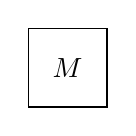
\begin{tikzpicture}[baseline=(current bounding box.center)]
    \draw (0,0) rectangle (1,1);
    \node at (0.5,0.5) {$M$};
  \end{tikzpicture}
  \approx
  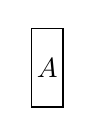
\begin{tikzpicture}[baseline=(current bounding box.center)]
    \draw (0,0) rectangle (0.4,1);
    \node at (0.2,0.5) {$A$};
  \end{tikzpicture}
  \cdot
  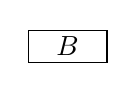
\begin{tikzpicture}[baseline=(current bounding box.center)]
    \draw (0,0) rectangle (1,0.4);
    \node at (0.5,0.2) {$B$};
  \end{tikzpicture}
\]

This problem can be translated into a numerical analysis problem of the following shape
\[
  \min_{A, B} \norm{M - AB}
\]
$A$ and $B$ can be obtained from eigenvectors of $M^TM$ and $MM^T$, but that's a huge, possibly dense matrix. So a more efficient way should be used, which also avoids the explicit formation of $M^TM$ and $MM^T$ because they need too much memory.\\

\noindent Efficiently solving this problem requires:
\begin{itemize}
    \item low-complexity computation (of course)
    \item avoiding ever explicitly forming $M^T M$ and $MM^T$ (too much memory)
    \item exploiting structure of $M$ (sparsity, similar columns, . . . )
    \item ensuring the solution is numerically stable
\end{itemize}

\subsubsection{Support vector machines}

Let us take a decision problem: given a set of values of many parameters (aka variables) ``label'' a person as ill or healthy, $y^i \in \{1, -1\}$.

The geometric intuition in two dimensions is given by \Cref{fig:19sett2}.
We would like to find the line that better splits the plane into two regions this  could help to diagnose the next patient.
The rationale here is to maximize the space between the line and the nearest points (called \textbf{margin}), in order to have a better accuracy.\\

\noindent The distance between the two hyperplanes $(w_+,w_0)$ and $(w_+,w^'_0)$ in \Cref{fig:19sett2} is:  $$|w_0 - w^'_0| / \norm{w_+}$$

\begin{itemize}
    \item Geometrically, the distance between these two hyperplanes is $\frac{2}{\norm{w_+}}$,  so to maximize the distance between the planes we want to minimize $\norm{w_+}$
    \item We can always take the hyperplane in the middle:
    $$ \Rightarrow w_+x^i + w_0 \geq 1 \; \;\text{if}\; \; y^i = 1 \; , \; w_+x^i + w_0 \leq -1 \; \;\text{if}\; \; y^i = -1$$
\end{itemize}




\addtwopics{0.4}{pics/19sett/svm4.pdf}{0.4}{pics/19sett/svm5.pdf}{There are many possible boundaries that can be chosen as a model using many angular coefficients. Our best guess is the one that maximizes the distance between the line and the nearest points.}{fig:19sett2}

\noindent So we have this optimization problem and the maximum-margin separating hyperplane (assuming any exists) is the solution of
\[
  {\min\limits_w \big\{\sqrnorm{w_+}~:~y^i( w_+ x^i + w_0 ) \geq 1, ~ i = 1, \ldots, m \big\}}
\]
       

In fact, what happens most of the times is that there is no such line. 
To overcome this issue we introduce the concept of ``penalty'' that accounts for the number of points that are misclassified.

\begin{definition}[SVM Primal problem]
\begin{equation}
\tag{SVM-P}
\begin{aligned}
& \min\limits_{w,\xi} & & {\sqrnorm{w_+} + C \sum\limits_{i=1}^m \xi_i}\\
& \text{s.t.} & &  y^i( w_+ x^i + w_0 ) \geq 1 - \xi_i \, , \, \xi_i \geq 0 \, ,  \, \forall i = 1, \ldots, m 
\end{aligned}    
\end{equation}
\end{definition}

This is the Support Vector Machine primal problem (SVM-P) a convex constrained problem with complex constraints and it's a multi-objective optimization problem.
Where $C$ is called \textbf{hyper-parameter} and there are the weighs violation of separation against margin.\\

This formula formalizes the intuition that the approximated function may have a greater norm and lead to a very small misclassification error, or it could be the other way round.
  Both these solutions are acceptable and their performances depend only on the problem.

This whole course has the aim of presenting some techniques for solving efficiently \textbf{convex quadratic problems}, as the ones presented above (SVM-P) or (SVM-D).\\

Whenever we are able to solve the multi-objective optimization problem we are also able to solve what is called the \textbf{dual problem}, which is formally defined as SPV-D and has the following shape in our case:
\begin{definition}[SVM Dual problem]
\begin{equation}
\tag{SVM-D}
\begin{aligned}
& \max\limits_{\alpha}  & &  \sum\limits_{i=1}^m \alpha_i - \frac{1}{2} \sum\limits_{i=1}^m \sum_{j=1}^m \alpha_i \ps{x^i}{x^j} \alpha_j\\
& \text{s.t.} & &  \sum\limits_{i=1}^m y^i \alpha_i = 0\\
& & & 0 \leq \alpha_i \leq C \, , \,  \forall i = 1, \ldots, m
\end{aligned}    
\end{equation}
\end{definition}

a convex constrained quadratic program, but with “simple constraints”. The idea is solve one problem by solving an apparently different one:
$$ \alpha^* \, \text{optimal for (SVM-D)} \Rightarrow w^*_+ = \sum_{i=1}^{m} \alpha_i^* y^i x^i \, \text{optimal for (SVM-P)} $$
Dual formulation $\Rightarrow$ kernel trick: input space $\rightsquigarrow$ (larger) feature space where points are hopefully “more linearly separable”
    $$ \ps{x^i}{x^j} \rightsquigarrow \ps{\phi(x^i)}{\phi(x^j)}$$

Feature space can be infinite-dimensional, provided that scalar product can be (efficiently) computed

\end{document}
